%%%%%%%%%%%%%%%%%%%%%%%%%%%%%%%%%%%%%%%%%%%%%%%%%%%%%%%%%%%%%%%%%%%%%%%%%%%%%%%%%%%%%%%%%%%%%%%%%%%
%%%%%%%%%%%%%%%%%%%%%%%%%%%%%%%%%%%%%%%%%%%%%%%%%%%%%%%%%%%%%%%%%%%%%%%%%%%%%%%%%%%%%%%%%%%%%%%%%%%
\chapter{Resultados}

%Como se mencion\'o previamente, este trabajo se ha basado en los registros de PSG de 6 adultos
%mayores con deterioro cognitivo (DC) y 3 sin este padecimiento. La calidad de deterioro
%cognitivo fue medida a trav\'es de una bater\'ia de pruebas neuropsicol\'ogicas;
%adicionalmente, se midi\'o su posible depresi\'on geri\'atrica. 
%En e cuadro \ref{sujetos} se resume esta informaci\'on.
%
%\begin{table}
%\centering
%\begin{tabular}{l|cc}
%Sujeto & Deterioro cogn. & Depresi\'on
%\\
%\hline
%MJNN &   &   \\
%RLMN & X &   \\
%JANA &   & X \\
%CLMN & X &   \\
%JGMN & X &   \\
%RRMN & X &   \\
%VCNN &   &   \\
%FGH  & X & ? \\
%GURM & ? & ? \\
%%& & \\
%%& & \\
%\end{tabular}
%\caption{Caracter\'isticas de los adultos mayores considerados en el estudio, en cuanto
%a deterioro cognitivo y depresi\'on geri\'atrica. 
%%Las dos primeras letras fueron dadas por sus nombre mientras que las \'ultimas dos son
%%mnemotecnias de sus caracter\'isticas: \textbf{M}= mean, \textbf{N}=normal, \textbf{A}=anormal.
%Para m\'as detalles consultar \cite{VazquezTagle16}}
%\label{sujetos}
%\end{table}

%Estos gr\'aficos muestran una distribuci\'ion temporal y pseudo-espacial 
%de las \'epocas que fueron clasificadas como {no-estacionarias} seg\'un el test PSR
%(ver seccipara m\'as detalles). 
%%M\'as que eso, esta distribuci\'on gr\'afica puede extenderse a otros an\'alisis.

En cada canal que conforma el PSG (EEG, EOG y EMG), 
cada una de las \'epocas consideradas fue clasificada como 
''\'Epoca Posiblemente Estacionaria'' (EPE) si no pudo ser rechazado la hip\'otesis de 
estacionariedad usando el test PSR ($\alpha = 0.05$), mientra que 
%el rechazo de esta misma 
%hip\'otesis es argumento ''suficiente'' para afirmar que el segmento de registro en cuenti\'on
%puede ser clasificado omo no.estacionario.
fue clasificado como ''No-estacionario'' en caso contrario. Variar el valor cr\'itico
para la clasificaci\'on no pareci\'o generar diferencias significativas.


La cantidad de \'epocas que no fueron para las cuales no es posible rechazar la hip\'otesis de
estacionariedad ($\alpha=0.05$)
clasificadas como ''Posiblemente Estacionarias'' (PE). 
La cantidad de \'epocas PE en cada individuo %con respecto a la cantidad total de \'epocas
durante el sue\~no MOR y no-MOR
muestra en las tablas \ref{total_gpos_mor}, \ref{total_gpos_nmor} y
\ref{total_gpos_total}; debido a que entre los sujetos hubo una gran variabilidad entre el tiempo 
que permanecieron en sue\~no MOR, se sugiri\'o comparar no el total de \'epocas PE sino
la proporci\'on --con respecto a la duraci\'on, medida en \'epocas-- de estas etapas, 
mustr\'andose estos resultados en las tablas \ref{gpos_mor}, \ref{gpos_nmor} y
\ref{gpos_total}. En estas \'ultimas tablas, se han calculado promedios y desviaciones
est\'andar muestrales entre los dos grupos que son comparados.

\begin{SidewaysFigure}
\centering
\begin{tabular}{c|ccccc|cccc|ccc}
& VCR & MJH & JAE & GHA? & MFGR?
& CLO & RLO & RRU & JGZ
& FGH & MGG & EMT \\
\hline
C3 &1154&228&57&1487&&107&299&589&104&31&325&133 \\
C4 &1076&211&42&1497&&79&290&610&110&17&339&162 \\
CZ &1082&210&38&1376&&93&255&581&117&16&318&132 \\
F3 &1019&116&14&28&&47&136&530&18&5&96&65 \\
F4 &1067&233&52&1233&&104&311&542&128&338&247&80 \\
F7 &1106&218&29&1366&&74&277&498&89&0&241&145 \\
F8 &960&203&46&1211&&80&208&427&100&0&220&70 \\
FP1 &1048&190&19&1305&&62&188&477&81&0&196&148 \\
FP2 &898&145&35&1207&&55&0&419&73&403&244&119 \\
FZ &981&132&29&1257&&53&171&313&73&0&234&95 \\
O1 &1066&230&46&1363&&105&330&532&140&0&298&152 \\
O2 &1074&351&127&1600&&184&288&570&341&90&556&265 \\
P3 &1295&266&35&633&&84&270&635&165&36&271&228 \\
P4 &1261&275&34&1065&&51&250&569&169&33&279&189 \\
PZ &1161&223&19&1360&&117&274&613&143&46&349&146 \\
T3 &1210&223&44&1472&&91&255&640&114&34&327&140 \\
T4 &1161&237&30&1363&&99&300&641&107&27&295&130 \\
T5 &1062&325&96&1626&&190&276&530&320&97&581&307 \\
T6 &1122&229&33&893&&128&208&499&161&46&221&155 \\
LOG &1181&202&22&1436&&52&224&595&128&16&206&127 \\
ROG &1313&233&1&697&&138&257&623&92&41&362&179 \\
EMG &1267&230&28&1072&&59&214&600&144&30&323&188 \\
\hline
Total&2584&1032&907&3281&&944&846&1244&1207&405&1030&555
\end{tabular}
\caption{Total de \'epocas PE clasificadas como sue\~no MOR 
(fase R) para cada
canal. %Se incluyen las medias y desviaciones est\'andar estimadas para los grupos 
%Control (izquierda) y PDC (centro).
}
\label{total_gpos_mor}
\end{SidewaysFigure}

\begin{SidewaysFigure}
\centering
\begin{tabular}{c|ccccc|cccc|ccc}
& VCR & MJH & JAE & GHA? & MFGR? 
& CLO & RLO & RRU & JGZ
& FGH & MGG & EMT \\
\hline
C3 &1048&201&41&1376&&99&249&524&101&28&285&116 \\
C4 &989&188&41&1372&&72&232&547&109&16&306&146 \\
CZ &999&185&37&1260&&86&221&519&115&13&289&115 \\
F3 &927&101&11&26&&28&116&501&18&5&91&63 \\
F4 &972&196&47&1136&&96&257&485&124&319&220&74 \\
F7 &1014&188&28&1256&&67&229&446&88&0&233&129 \\
F8 &899&181&45&1141&&77&180&407&100&0&214&67 \\
FP1 &966&162&19&1194&&56&152&464&81&0&194&134 \\
FP2 &848&133&23&1079&&54&0&404&73&381&243&110 \\
FZ &922&121&28&1160&&52&151&297&73&0&232&91 \\
O1 &972&198&44&1259&&90&273&470&134&0&271&135 \\
O2 &1022&317&124&1462&&179&272&548&341&89&541&250 \\
P3 &1163&228&34&602&&79&227&563&163&31&239&206 \\
P4 &1138&238&33&991&&48&206&508&166&32&255&175 \\
PZ &1057&194&19&1261&&109&225&552&142&45&313&128 \\
T3 &1106&195&44&1359&&85&214&579&111&28&301&124 \\
T4 &1055&210&30&1258&&91&254&574&107&24&278&115 \\
T5 &1002&292&95&1493&&178&263&501&319&97&553&288 \\
T6 &1003&192&32&838&&113&163&454&161&42&174&141 \\
LOG &1072&169&22&1322&&46&182&535&127&16&193&110 \\
ROG &1198&190&1&665&&125&209&560&87&37&304&160 \\
EMG &1159&197&28&1001&&54&178&531&141&30&301&172 \\
\hline
Total&2384&896&736&3014&&812&747&1130&1174&383&864&508
\end{tabular}
\caption{Total  de \'epocas PE dentro del registro pero que no fueron clasificadas
como MOR (fases W y N) para cada
canal. %Se incluyen las medias y desviaciones est\'andar estimadas para los grupos 
%Control (izquierda) y PDC (centro).
}
\label{total_gpos_nmor}
\end{SidewaysFigure}

\begin{SidewaysFigure}
\centering
\begin{tabular}{c|ccccc|cccc|ccc}
& VCR & MJH & JAE & GHA? & MFGR?
& CLO & RLO & RRU & JGZ
& FGH & MGG & EMT \\
\hline
C3 &106&27&16&111&&8&50&65&3&3&40&17 \\
C4 &87&23&1&125&&7&58&63&1&1&33&16 \\
CZ &83&25&1&116&&7&34&62&2&3&29&17 \\
F3 &92&15&3&2&&19&20&29&0&0&5&2 \\
F4 &95&37&5&97&&8&54&57&4&19&27&6 \\
F7 &92&30&1&110&&7&48&52&1&0&8&16 \\
F8 &61&22&1&70&&3&28&20&0&0&6&3 \\
FP1 &82&28&0&111&&6&36&13&0&0&2&14 \\
FP2 &50&12&12&128&&1&0&15&0&22&1&9 \\
FZ &59&11&1&97&&1&20&16&0&0&2&4 \\
O1 &94&32&2&104&&15&57&62&6&0&27&17 \\
O2 &52&34&3&138&&5&16&22&0&1&15&15 \\
P3 &132&38&1&31&&5&43&72&2&5&32&22 \\
P4 &123&37&1&74&&3&44&61&3&1&24&14 \\
PZ &104&29&0&99&&8&49&61&1&1&36&18 \\
T3 &104&28&0&113&&6&41&61&3&6&26&16 \\
T4 &106&27&0&105&&8&46&67&0&3&17&15 \\
T5 &60&33&1&133&&12&13&29&1&0&28&19 \\
T6 &119&37&1&55&&15&45&45&0&4&47&14 \\
LOG &109&33&0&114&&6&42&60&1&0&13&17 \\
ROG &115&43&0&32&&13&48&63&5&4&58&19 \\
EMG &108&33&0&71&&5&36&69&3&0&22&16 \\
\hline
Total&200&127&171&267&&132&99&114&33&22&166&47
\end{tabular}
\caption{Total de \'epocas PE registradas
(todas las fases) para cada
canal. 
%Se incluyen las medias y desviaciones est\'andar estimadas para los grupos 
%Control (izquierda) y PDC (centro).
}
\label{total_gpos_total}
\end{SidewaysFigure}






%\begin{comment}
\begin{SidewaysFigure}
\centering
\begin{tabular}{c||ccccc|cc||cccc|cc||ccc}
& VCR & MJH & JAE & GHA? & MFGR? &$\widehat{\mu}$ & $\widehat{\sigma}$
& CLO & RLO & RRU & JGZ &$\widehat{\mu}$ & $\widehat{\sigma}$
& FGH & MGG & EMT \\
\hline
 C3 & 0.082    & 0.142    & 0.047    & 0.189    && 0.115    & 0.063    & 0.045    & 0.354    & 0.421    & 0.030    & 0.213    & 0.204    & 0.091    & 0.169    & 0.191     \\
 C4 & 0.096    & 0.126    & 0.006    & 0.126    && 0.089    & 0.057    & 0.030    & 0.404    & 0.132    & -      & 0.141    & 0.184    & 0.045    & 0.139    & 0.213     \\
 CZ & 0.027    & 0.126    & 0.006    & 0.095    && 0.063    & 0.056    & 0.038    & 0.222    & 0.105    & 0.030    & 0.099    & 0.089    & 0.045    & 0.078    & 0.255     \\
 F3 & 0.068    & 0.181    & 0.018    & 0.147    && 0.104    & 0.074    & 0.053    & 0.434    & 0.079    & 0.091    & 0.164    & 0.181    & 0.273    & 0.084    & 0.085     \\
 F4 & 0.151    & 0.181    & -      & 0.168    && 0.125    & 0.084    & 0.045    & 0.364    & 0.132    & -      & 0.135    & 0.162    & -      & 0.024    & 0.319     \\
 F7 & 0.068    & 0.118    & 0.006    & 0.232    && 0.106    & 0.095    & 0.008    & 0.182    & -      & -      & 0.047    & 0.090    & -      & 0.012    & 0.043     \\
 F8 & 0.055    & 0.087    & -      & 0.242    && 0.096    & 0.104    & 0.030    & 0.232    & 0.026    & -      & 0.072    & 0.108    & -      & 0.012    & 0.234     \\
 FP1 & 0.027    & 0.055    & 0.058    & 0.253    && 0.098    & 0.104    & -      & -      & 0.026    & -      & 0.007    & 0.013    & 1.000    & -      & 0.170     \\
 FP2 & 0.014    & 0.047    & 0.006    & 0.105    && 0.043    & 0.045    & 0.008    & 0.152    & 0.026    & -      & 0.046    & 0.071    & -      & 0.006    & 0.085     \\
 FZ & 0.151    & 0.142    & 0.012    & 0.126    && 0.108    & 0.065    & 0.053    & 0.384    & 0.053    & 0.061    & 0.138    & 0.164    & -      & 0.120    & 0.298     \\
 O1 & 0.137    & 0.157    & -      & 0.284    && 0.145    & 0.116    & 0.015    & 0.253    & 0.237    & 0.061    & 0.141    & 0.121    & 0.227    & 0.108    & 0.277     \\
 O2 & 0.178    & 0.181    & -      & 0.274    && 0.158    & 0.114    & 0.023    & 0.343    & 0.237    & 0.030    & 0.158    & 0.158    & 0.045    & 0.072    & 0.106     \\
 P3 & 0.082    & 0.134    & -      & 0.263    && 0.120    & 0.110    & 0.038    & 0.333    & 0.211    & -      & 0.145    & 0.155    & 0.045    & 0.145    & 0.234     \\
 P4 & 0.055    & 0.150    & -      & 0.295    && 0.125    & 0.129    & 0.030    & 0.273    & 0.132    & 0.030    & 0.116    & 0.115    & 0.182    & 0.090    & 0.234     \\
 PZ & 0.055    & 0.118    & -      & 0.221    && 0.098    & 0.095    & 0.030    & 0.323    & 0.105    & -      & 0.115    & 0.146    & 0.045    & 0.048    & 0.149     \\
 T3 & 0.137    & 0.228    & -      & 0.274    && 0.160    & 0.121    & 0.076    & 0.343    & 0.105    & -      & 0.131    & 0.148    & 0.091    & 0.175    & 0.149     \\
 T4 & 0.164    & 0.157    & -      & 0.116    && 0.109    & 0.076    & 0.023    & 0.354    & 0.158    & 0.030    & 0.141    & 0.155    & -      & 0.060    & 0.277     \\
 T5 & 0.137    & 0.205    & -      & 0.211    && 0.138    & 0.098    & 0.038    & 0.343    & 0.132    & 0.061    & 0.143    & 0.139    & 0.091    & 0.187    & 0.319     \\
 T6 & 0.205    & 0.142    & -      & 0.263    && 0.153    & 0.113    & 0.023    & 0.242    & 0.105    & 0.061    & 0.108    & 0.096    & -      & 0.054    & 0.234     \\
 LOG & 0.082    & 0.157    & 0.018    & 0.263    && 0.130    & 0.106    & 0.038    & 0.111    & 0.053    & -      & 0.050    & 0.046    & 0.045    & 0.048    & 0.277     \\
 ROG & 0.082    & 0.165    & 0.006    & 0.316    && 0.142    & 0.133    & 0.068    & 0.071    & 0.105    & 0.030    & 0.069    & 0.031    & -      & 0.114    & 0.340     \\
 EMG & 0.192    & 0.087    & 0.012    & -      && 0.073    & 0.088    & 0.106    & 0.162    & 0.105    & -      & 0.093    & 0.068    & -      & 0.018    & 0.021     \\
\end{tabular}
\caption{Proporci\'on estimada de \'epocas PE respecto al total de \'epocas MOR 
(fase R) para cada
canal. Se incluyen las medias y desviaciones est\'andar estimadas para los grupos 
Control (izquierda) y PDC (centro).}
\label{gpos_mor}
\end{SidewaysFigure}

\begin{SidewaysFigure}
\centering
\begin{tabular}{c||ccccc|cc||cccc|cc||ccc}
& VCR & MJH & JAE & GHA? & MFGR? &$\widehat{\mu}$ & $\widehat{\sigma}$
& CLO & RLO & RRU & JGZ &$\widehat{\mu}$ & $\widehat{\sigma}$
& FGH & MGG & EMT \\
\hline
 C3 & 0.237    & 0.149    & 0.030    & 0.160    && 0.144    & 0.086    & 0.068    & 0.205    & 0.202    & 0.048    & 0.131    & 0.085    & 0.042    & 0.233    & 0.142     \\
 C4 & 0.213    & 0.143    & 0.033    & 0.146    && 0.134    & 0.075    & 0.044    & 0.181    & 0.250    & 0.040    & 0.129    & 0.104    & 0.018    & 0.240    & 0.181     \\
 CZ & 0.212    & 0.145    & 0.030    & 0.100    && 0.122    & 0.077    & 0.067    & 0.194    & 0.184    & 0.053    & 0.124    & 0.075    & 0.021    & 0.208    & 0.138     \\
 F3 & 0.213    & 0.148    & 0.037    & 0.136    && 0.134    & 0.073    & 0.070    & 0.234    & 0.210    & 0.058    & 0.143    & 0.092    & 0.279    & 0.166    & 0.091     \\
 F4 & 0.228    & 0.146    & 0.024    & 0.131    && 0.133    & 0.084    & 0.050    & 0.181    & 0.213    & 0.042    & 0.121    & 0.088    & -      & 0.159    & 0.179     \\
 F7 & 0.201    & 0.151    & 0.039    & 0.191    && 0.146    & 0.074    & 0.055    & 0.150    & 0.181    & 0.049    & 0.109    & 0.066    & -      & 0.176    & 0.079     \\
 F8 & 0.199    & 0.136    & 0.019    & 0.146    && 0.125    & 0.076    & 0.050    & 0.129    & 0.229    & 0.041    & 0.112    & 0.087    & -      & 0.148    & 0.181     \\
 FP1 & 0.207    & 0.083    & 0.018    & 0.100    && 0.102    & 0.078    & 0.042    & -      & 0.189    & 0.037    & 0.067    & 0.083    & 0.995    & 0.196    & 0.142     \\
 FP2 & 0.198    & 0.091    & 0.027    & 0.106    && 0.105    & 0.070    & 0.041    & 0.133    & 0.069    & 0.037    & 0.070    & 0.044    & -      & 0.169    & 0.110     \\
 FZ & 0.216    & 0.148    & 0.034    & 0.144    && 0.136    & 0.075    & 0.068    & 0.218    & 0.242    & 0.055    & 0.146    & 0.098    & -      & 0.205    & 0.171     \\
 O1 & 0.256    & 0.192    & 0.023    & 0.272    && 0.186    & 0.114    & 0.059    & 0.201    & 0.245    & 0.082    & 0.147    & 0.090    & 0.052    & 0.162    & 0.242     \\
 O2 & 0.211    & 0.182    & 0.023    & 0.224    && 0.160    & 0.093    & 0.039    & 0.182    & 0.186    & 0.090    & 0.124    & 0.072    & 0.057    & 0.186    & 0.209     \\
 P3 & 0.222    & 0.135    & 0.012    & 0.266    && 0.159    & 0.112    & 0.089    & 0.197    & 0.287    & 0.081    & 0.163    & 0.098    & 0.076    & 0.245    & 0.130     \\
 P4 & 0.228    & 0.150    & 0.034    & 0.229    && 0.161    & 0.092    & 0.069    & 0.181    & 0.293    & 0.062    & 0.151    & 0.109    & 0.047    & 0.238    & 0.144     \\
 PZ & 0.198    & 0.145    & 0.019    & 0.199    && 0.140    & 0.085    & 0.070    & 0.224    & 0.298    & 0.050    & 0.160    & 0.120    & 0.039    & 0.205    & 0.128     \\
 T3 & 0.230    & 0.155    & 0.027    & 0.212    && 0.156    & 0.092    & 0.100    & 0.150    & 0.213    & 0.087    & 0.137    & 0.057    & 0.070    & 0.133    & 0.175     \\
 T4 & 0.230    & 0.134    & 0.015    & 0.180    && 0.140    & 0.092    & 0.032    & 0.147    & 0.298    & 0.074    & 0.138    & 0.117    & 0.026    & 0.141    & 0.138     \\
 T5 & 0.277    & 0.161    & -      & 0.248    && 0.172    & 0.124    & 0.096    & 0.183    & 0.277    & 0.052    & 0.152    & 0.099    & 0.050    & 0.241    & 0.215     \\
 T6 & 0.277    & 0.164    & 0.023    & 0.193    && 0.164    & 0.106    & 0.047    & 0.158    & 0.261    & 0.072    & 0.134    & 0.097    & 0.047    & 0.242    & 0.234     \\
 LOG & 0.299    & 0.248    & 0.118    & 0.263    && 0.232    & 0.079    & 0.177    & 0.248    & 0.340    & 0.192    & 0.239    & 0.074    & 0.131    & 0.506    & 0.352     \\
 ROG & 0.299    & 0.227    & 0.091    & 0.307    && 0.231    & 0.100    & 0.155    & 0.240    & 0.293    & 0.192    & 0.220    & 0.060    & 0.175    & 0.527    & 0.413     \\
 EMG & 0.119    & 0.069    & 0.005    & 0.002    && 0.049    & 0.056    & 0.025    & 0.110    & 0.293    & 0.009    & 0.109    & 0.130    & 0.003    & 0.064    & 0.083   
\end{tabular}
\caption{Proporci\'on estimada de \'epocas PE respecto al total de \'epocas no-MOR 
(fases W y N) para cada
canal. Se incluyen las medias y desviaciones est\'andar estimadas para los grupos 
Control (izquierda) y PDC (centro).}
\label{gpos_nmor}
\end{SidewaysFigure}

\begin{SidewaysFigure}
\centering
\begin{tabular}{c||ccccc|cc||cccc|cc||ccc}
& VCR & MJH & JAE & GHA? & MFGR? &$\widehat{\mu}$ & $\widehat{\sigma}$
& CLO & RLO & RRU & JGZ &$\widehat{\mu}$ & $\widehat{\sigma}$
& FGH & MGG & EMT \\
\hline
 C3 & 0.224    & 0.148    & 0.033    & 0.163    && 0.142    & 0.080    & 0.065    & 0.222    & 0.222    & 0.047    & 0.139    & 0.096    & 0.044    & 0.222    & 0.146    \\
 C4 & 0.203    & 0.141    & 0.028    & 0.145    && 0.129    & 0.073    & 0.042    & 0.207    & 0.239    & 0.039    & 0.132    & 0.106    & 0.020    & 0.223    & 0.184    \\
 CZ & 0.196    & 0.142    & 0.025    & 0.100    && 0.116    & 0.072    & 0.063    & 0.197    & 0.176    & 0.052    & 0.122    & 0.075    & 0.022    & 0.187    & 0.148    \\
 F3 & 0.201    & 0.152    & 0.033    & 0.137    && 0.131    & 0.071    & 0.068    & 0.258    & 0.198    & 0.059    & 0.146    & 0.098    & 0.279    & 0.152    & 0.090    \\
 F4 & 0.222    & 0.150    & 0.020    & 0.134    && 0.132    & 0.084    & 0.050    & 0.202    & 0.205    & 0.041    & 0.124    & 0.092    & -      & 0.137    & 0.191    \\
 F7 & 0.189    & 0.147    & 0.033    & 0.195    && 0.141    & 0.075    & 0.049    & 0.154    & 0.164    & 0.048    & 0.104    & 0.064    & -      & 0.150    & 0.076    \\
 F8 & 0.187    & 0.130    & 0.015    & 0.155    && 0.122    & 0.075    & 0.048    & 0.141    & 0.210    & 0.040    & 0.110    & 0.081    & -      & 0.126    & 0.186    \\
 FP1 & 0.192    & 0.079    & 0.025    & 0.113    && 0.102    & 0.070    & 0.036    & -      & 0.174    & 0.036    & 0.062    & 0.077    & 0.995    & 0.164    & 0.144    \\
 FP2 & 0.182    & 0.085    & 0.023    & 0.106    && 0.099    & 0.066    & 0.036    & 0.135    & 0.065    & 0.036    & 0.068    & 0.046    & -      & 0.143    & 0.108    \\
 FZ & 0.210    & 0.147    & 0.030    & 0.143    && 0.133    & 0.075    & 0.066    & 0.238    & 0.225    & 0.056    & 0.146    & 0.099    & -      & 0.191    & 0.182    \\
 O1 & 0.246    & 0.188    & 0.019    & 0.273    && 0.181    & 0.114    & 0.053    & 0.207    & 0.244    & 0.081    & 0.146    & 0.093    & 0.062    & 0.153    & 0.245    \\
 O2 & 0.208    & 0.182    & 0.019    & 0.229    && 0.159    & 0.096    & 0.037    & 0.201    & 0.191    & 0.089    & 0.129    & 0.080    & 0.057    & 0.168    & 0.200    \\
 P3 & 0.210    & 0.135    & 0.010    & 0.265    && 0.155    & 0.111    & 0.082    & 0.213    & 0.280    & 0.079    & 0.163    & 0.100    & 0.074    & 0.229    & 0.139    \\
 P4 & 0.214    & 0.150    & 0.028    & 0.235    && 0.157    & 0.093    & 0.064    & 0.191    & 0.278    & 0.061    & 0.149    & 0.105    & 0.054    & 0.215    & 0.151    \\
 PZ & 0.186    & 0.141    & 0.015    & 0.201    && 0.136    & 0.084    & 0.065    & 0.235    & 0.280    & 0.049    & 0.157    & 0.118    & 0.040    & 0.180    & 0.130    \\
 T3 & 0.222    & 0.164    & 0.022    & 0.218    && 0.156    & 0.093    & 0.096    & 0.173    & 0.203    & 0.085    & 0.139    & 0.058    & 0.072    & 0.140    & 0.173    \\
 T4 & 0.224    & 0.137    & 0.012    & 0.175    && 0.137    & 0.091    & 0.031    & 0.171    & 0.285    & 0.073    & 0.140    & 0.113    & 0.025    & 0.128    & 0.150    \\
 T5 & 0.265    & 0.167    & -      & 0.245    && 0.169    & 0.120    & 0.088    & 0.202    & 0.263    & 0.052    & 0.151    & 0.098    & 0.052    & 0.232    & 0.223    \\
 T6 & 0.271    & 0.161    & 0.019    & 0.199    && 0.162    & 0.106    & 0.043    & 0.168    & 0.246    & 0.071    & 0.132    & 0.093    & 0.044    & 0.212    & 0.234    \\
 LOG & 0.281    & 0.236    & 0.099    & 0.263    && 0.220    & 0.082    & 0.158    & 0.232    & 0.314    & 0.186    & 0.222    & 0.068    & 0.126    & 0.432    & 0.346    \\
 ROG & 0.281    & 0.219    & 0.075    & 0.307    && 0.221    & 0.104    & 0.143    & 0.220    & 0.275    & 0.187    & 0.206    & 0.056    & 0.165    & 0.460    & 0.407    \\
 EMG & 0.125    & 0.071    & 0.007    & 0.002    && 0.051    & 0.059    & 0.036    & 0.116    & 0.275    & 0.008    & 0.109    & 0.120    & 0.002    & 0.056    & 0.077    
\end{tabular}
\caption{Proporci\'on estimada de \'epocas PE respecto al total de \'epocas registradas
(todas las fases) para cada
canal. Se incluyen las medias y desviaciones est\'andar estimadas para los grupos 
Control (izquierda) y PDC (centro).}
\label{gpos_total}
\end{SidewaysFigure}
%\end{comment}

\begin{SidewaysFigure}
\centering
\begin{tabular}{c||ccccc||cccc||ccc}
& VCR & MJH & JAE & GHA? & MFGR? & CLO & RLO & RRU & JGZ & FGH & MGG & EMT \\
\hline
 C3 & *** &&&&&& *** & ** &&&& \\
 C4 & ** &&&&&& *** &&&& ** & \\
 CZ & *** &&&&&&&&&& *** & *  \\
 F3 & *** &&&&&& *** &&&& ** & \\
 F4 &&&&&&& *** &&&& *** & *  \\
 F7 & ** && * &&& * && ** &&& *** & \\
 F8 & *** &&& ** &&& ** & ** &&& *** & \\
 FP1 & *** && ** & *** && * && ** &&& *** & \\
 FP2 & *** &&&&&&&&&& *** & \\
 FZ &&&&&&& *** & ** &&& ** & *  \\
 O1 & ** &&&&& * &&&& ** && \\
 O2 &&&&&&& *** &&&& *** & \\
 P3 & ** &&&&&& *** &&&& ** & \\
 P4 & *** && * &&&& * & * && ** & *** & \\
 PZ & *** &&&&&& * & ** &&& *** & \\
 T3 && * & * &&&& *** &&&&& \\
 T4 &&&&&&& *** &&&& ** & **  \\
 T5 & ** &&&&& * & *** &&&&& \\
 T6 &&&&&&& * & * &&& *** & \\
 LOG & *** & * & *** &&& *** & *** & *** & ** && *** & \\
 ROG & *** && *** &&& ** & *** & ** & ** & * & *** & \\
 EMG &&&&&& *** && ** &&& * &
\end{tabular}
\caption{Diferencias significativas en la comparaci\'on entre proporci\'on
de \'epocas PE en sue\~no MOR (fase R) y no-MOR (fases W y N)}
\label{comparacion_mor_vs_total}
\end{SidewaysFigure}

Como un primer an\'alisis, para cada sujeto y en cada canal 
se compar\'o la proporci\'on de \'epocas PE en sue\~no MOR contra el registro completo;
el fin de ello es verificar si el sue\~no MOR --entendido como muestra no-aleatoria
del sue\~no-- tiene propiedades similares o no, y si \'esta similaridad pudiera estar
relacionada con el PDC del paciente. 
Las comparaciones se llevaron a cabo usando una prueba $\chi^{2}$ para proporciones,
y los resultados se muestran en la tabla \ref{comparacion_mor_vs_total}.
Se encontr\'o que no hay una relaci\'on clara entre el estado de salud del sujeto y
la aparici\'on de diferencias significativas entre estas proporciones; en la secci\'on
de discusi\'on se mencionan algunos datos que se ''recuperaron'' de este an\'alisis.

Posteriormente se procedi\'o a comparar, por cada canal, si la proporci\'on de \'epocas PE
presenta diferencias significativas entre los grupos. Esta comparaci\'on se realiz\'o tomando
en cuenta las \'epocas de sue\~no MOR, de sue\~no no-MOR, y el registro completo 
--ver, respectivamente, tablas \ref{gpos_mor}, \ref{gpos_nmor}, \ref{gpos_total}.
Para una mejor visualizaci\'on de estos, se han graficado
% que representan
%las proporciones respectivas de cada sujeto --para ambos grupos.
en la figura \ref{comparacion_graf}
los datos de las tablas \ref{gpos_mor}, \ref{gpos_nmor} y
\ref{gpos_total}.

\begin{figure}
\centering
\subfloat[Comparaci\'on entre \'epocas MOR (fase R)]{
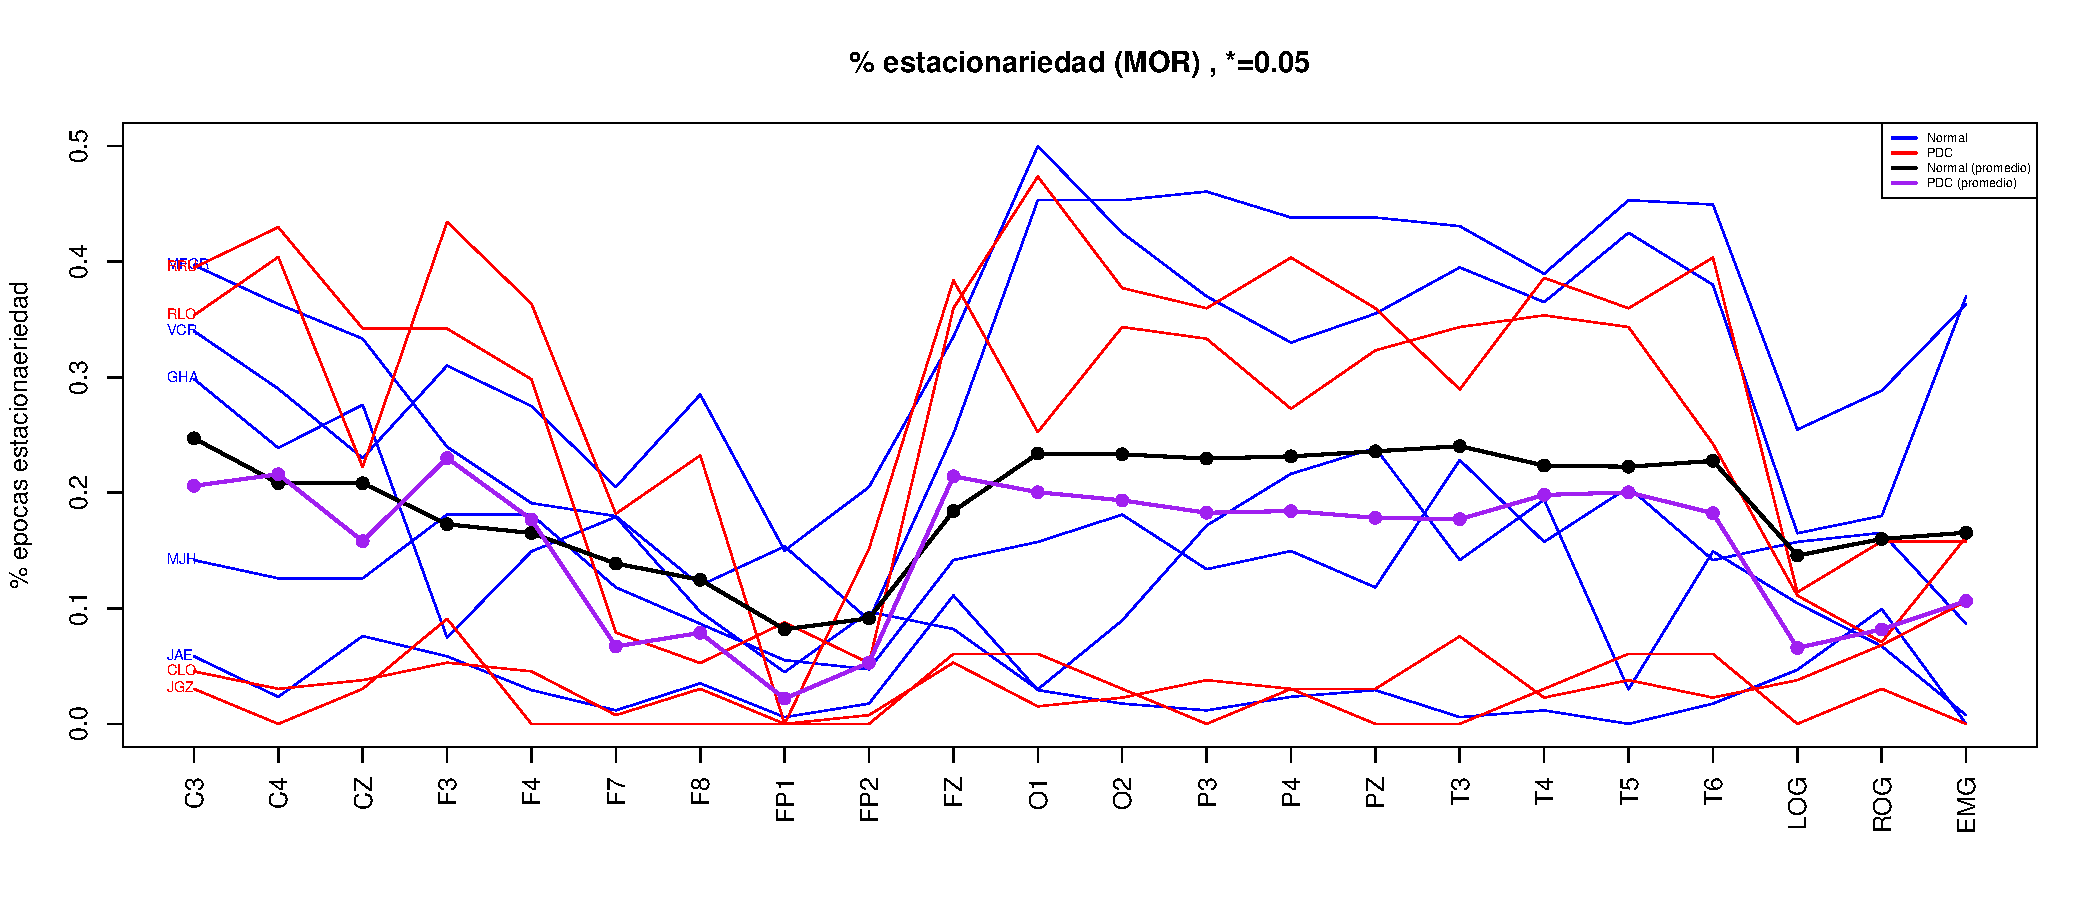
\includegraphics[width=0.9\linewidth]
{./material170331/Comparacion_gpos_MOR.pdf} 
}\\
\subfloat[Comparaci\'on entre \'epocas no-MOR (fases W y N)]{
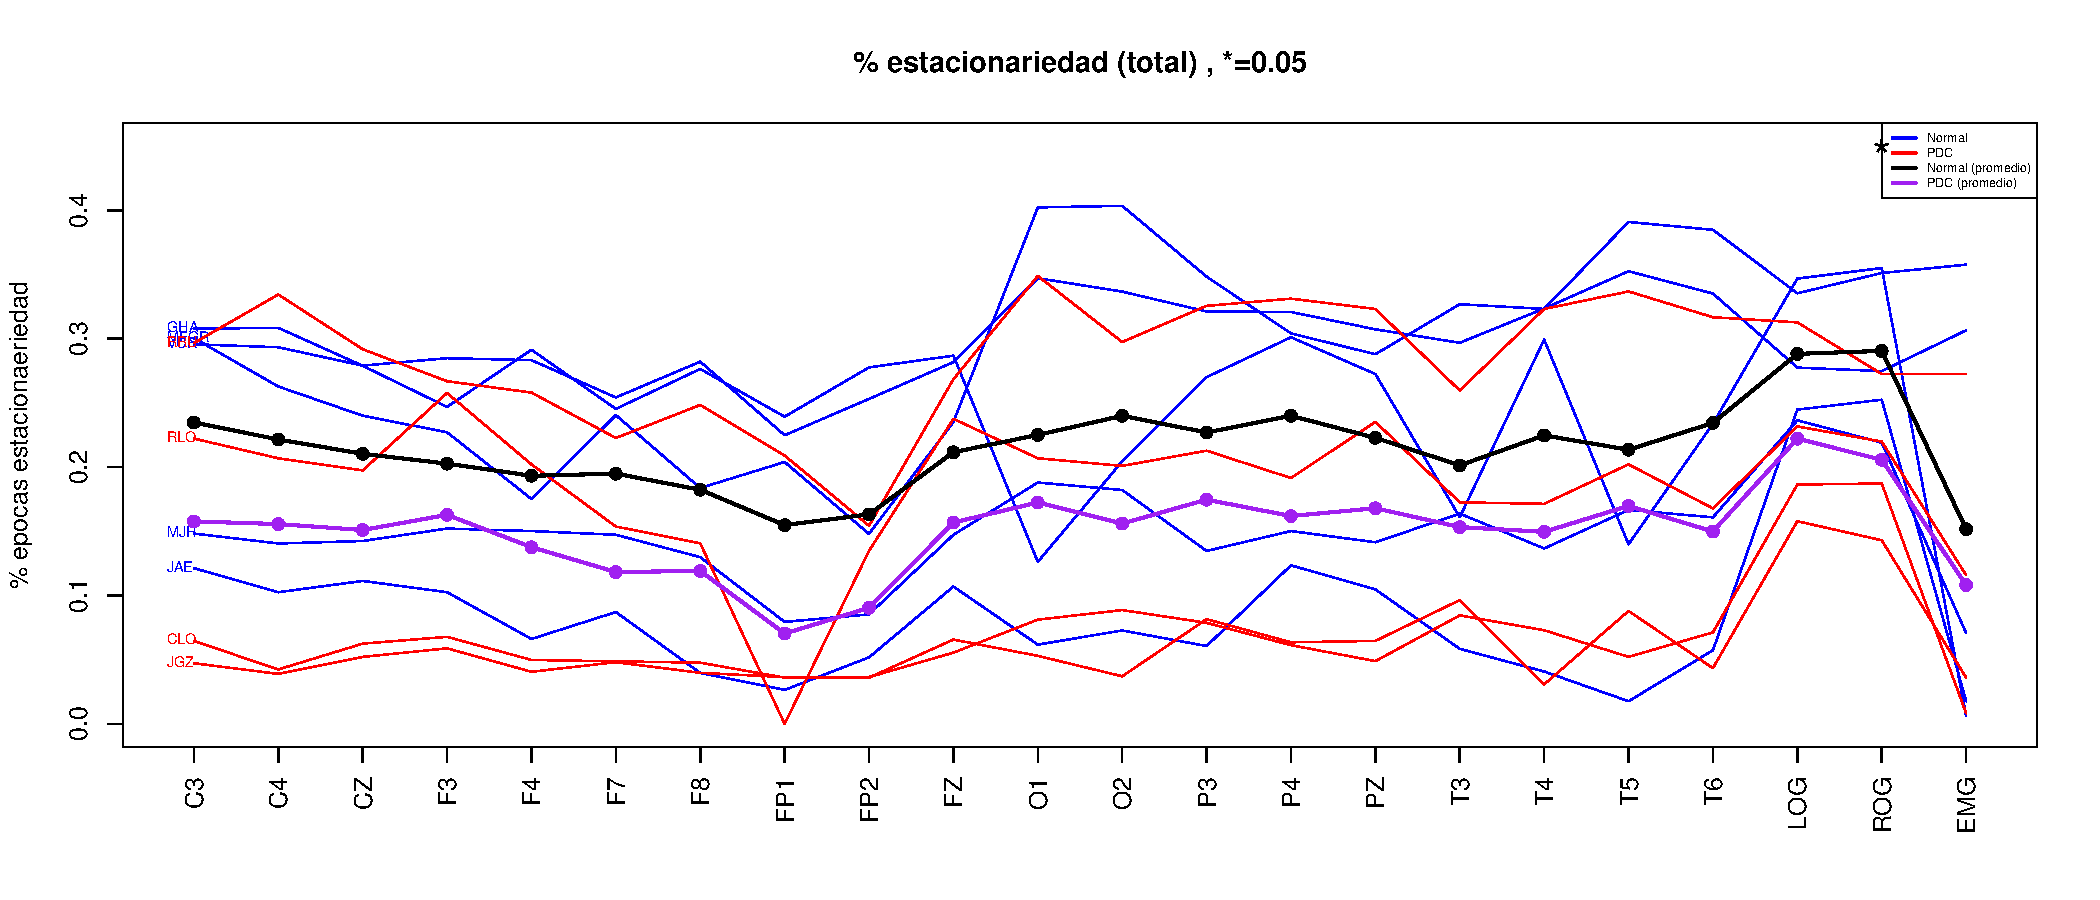
\includegraphics[width=0.9\linewidth]
{./material170331/Comparacion_gpos_NMOR.pdf} 
}\\
\subfloat[Comparaci\'on entre el total de \'epocas registradas]{
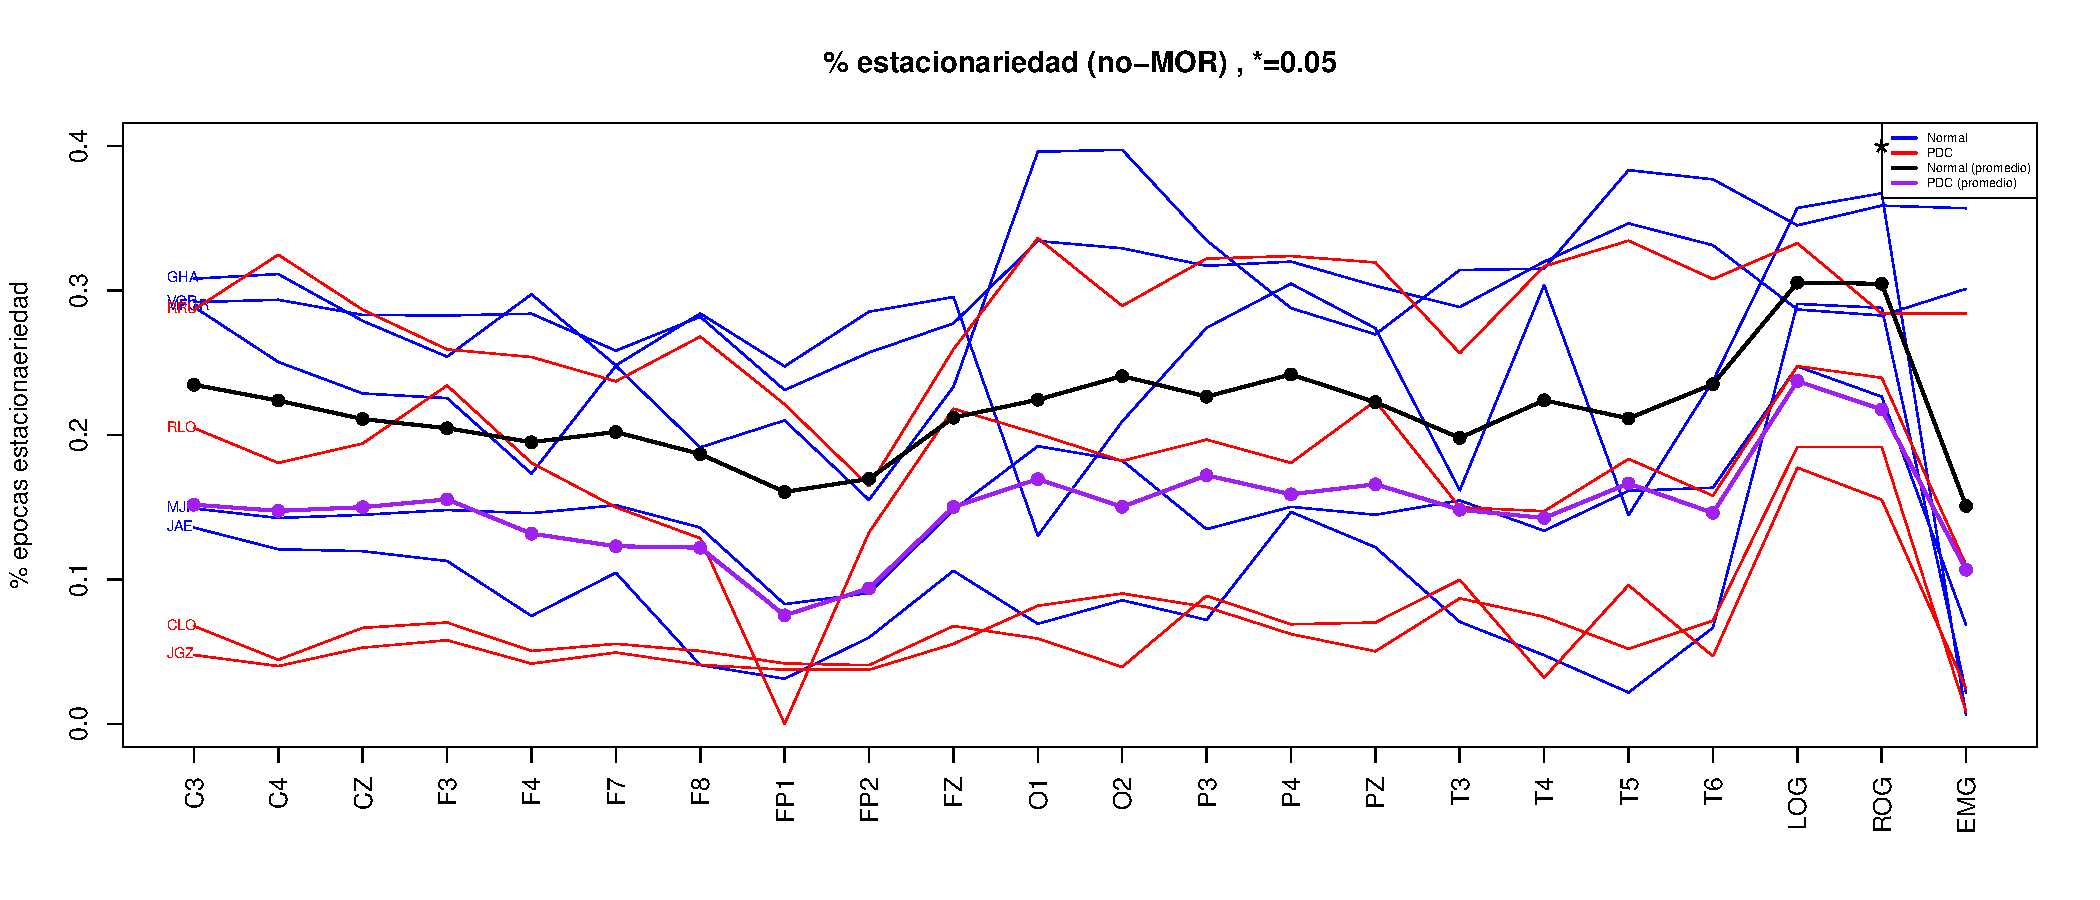
\includegraphics[width=0.9\linewidth]
{./material170331/Comparacion_gpos_TOT.pdf} 
}\\
\caption{Comparaci\'on entre las proporciones de \'epocas PE en diferentes
etapas de sue\~no; 
se sobrelapan en diferentes colores los sujetos con y sin PDC.}
\label{comparacion_graf}
\end{figure}

La comparaci\'on per se se llev\'o a cabo usando las pruebas %no param\'etrica
$t$ de Student y $U$ de Mann-Whitney-Wilcoxon.
El primer test arroja diferencias significativas para los canales LOG, ROG y EMG, mientras que
el segundo indica que no hay diferencias significativas. 

Debido a que los canales
donde se hallaron diferencias significativas no corresponden a registros de actividad
cerebral, se considera que \textbf{esta caracter\'istica no proporciona evidencias
suficientes sobre diferencias significativas entre adultos mayores con y sin PDC diagnosticado}.
Este resultado es clave en el desarrollo de este trabajo.

%\begin{table}
%\centering
%\begin{tabular}{}
%
%\end{tabular}
%\caption{Proporci\'on estimada de \'epocas PE respecto al total de \'epocas MOR 
%(fase R) en cada
%canal, para el grupo \textit{Normal}.}
%\label{gpo_NN_mor}
%\end{table}

%%%%%%%%%%%%%%%%%%%%%%%%%%%%%%%%%%%%%%%%%%%%%%%%%%%%%%%%%%%%%%%%%%%%%%%%%%%%%%%%%%%%%%%%%%%%%%%%%%%
%%%%%%%%%%%%%%%%%%%%%%%%%%%%%%%%%%%%%%%%%%%%%%%%%%%%%%%%%%%%%%%%%%%%%%%%%%%%%%%%%%%%%%%%%%%%%%%%%%%